\documentclass{article}
\usepackage[utf8]{inputenc}
\usepackage{hyperref}
\usepackage{setspace} %for controlling line spacing
\usepackage{graphicx}
% Optional: to have the image path relative to the .tex file
\graphicspath{ {./images/} }

\title{Enhancing the SAML 2.0 Protocol — Toward Certificate-Decoupled Identity Federation\\ \textit{A Path to SAML 3.0}}
\author{
Pushkar Raj, Lead Software Engineer - IAM \\ 
\href{https://orcid.org/0009-0002-8444-0136}{\texttt{ORCID: 0009-0002-8444-0136}} \\
\href{mailto:pushkarraj9099@gmail.com}pushkarraj9099@gmail.com
\and
Sandeep R, Staff Software Engineer - IAM \\ 
\href{mailto:sandeep.r79@gmail.com}sandeep.r79@gmail.com
}
\date{\today}
\begin{document}

\maketitle

\section*{Executive Summary}
SAML 2.0 has established itself as a cornerstone for federated identity management, enabling secure communication between Identity Providers (IdPs) and Service Providers (SPs). While the protocol supports robust authentication and assertion mechanisms, it ties signing certificates directly to SP configurations, requiring manual interventions for certificate rotations.

This tight coupling creates significant operational inefficiencies during certificate expiration or renewal processes. Organizations often face service disruptions, misconfigurations, and delays due to the manual synchronization required by both IdP and SP administrators.

To address these challenges, we propose a Certificate Abstraction Layer (CAL), a mechanism to decouple certificate management from the SAML authentication workflow. CAL introduces a dynamic \texttt{certificateID} association model, enabling SPs to reference certificates indirectly via base64-encoded thumbprints. A centralized certificate metadata endpoint hosted by IdPs will facilitate automated discovery and validation. This also include caching mechanisms on SPs for certificate metadata and extensibility of federation metadata for seamless CAL integration.

The proposed enhancement reduces human oversight, improves scalability, and fosters automation-friendly workflows. CAL offers backward compatibility, allowing organizations to migrate gradually without disrupting legacy federation setups.

\section*{Background and Problem Statement}
\textbf{Current State of SAML 2.0:}  
SAML federations rely on tightly coupled configurations between SPs and signing certificates. Certificates embedded in metadata ensure integrity in communications, but any updates—whether due to expiration or rotation—require manual intervention on both sides.

\textbf{Challenges:}
\begin{itemize}
    \item \textbf{Key Rotation Effort:} Administrators must manually synchronize certificate updates on both IdP and SP configurations during rotation, creating delays and scalability bottlenecks.
    \item \textbf{Downtime Risk:} Risks of service disruptions caused by misconfigured certificates are exacerbated when coordination failures occur.
    \item \textbf{Scalability and Automation Obstacles:} Static certificate references prevent agile federation onboarding or automation, reducing SAML’s suitability in dynamic environments like multi-cloud and DevOps workflows.
\end{itemize}

Without a mechanism to abstract certificate management, enterprises struggle with increased administrative overhead and slower adoption of cloud or hybrid architectures.

\subsection*{Source Reference}
This work references the SAML standard as defined by OASIS. For more details on SAML, see the official documentation at \href{https://www.oasis-open.org/standard/saml/}{OASIS SAML Standard Documentation}.


\section*{Use Cases Affected}
\begin{itemize}
    \item \textbf{Frequent Key Rotations:} Enterprises that frequently renew certificates for compliance or security reasons.
    \item \textbf{Dynamic Multi-Cloud Federation:} Hybrid deployments with dynamic authentication setups.
    \item \textbf{DevOps Workflows:} Environments requiring rapid provisioning and de-provisioning of federations.
    \item \textbf{Regulatory Compliance:} Industries that demand frequent cryptographic updates for audit compliance and security mandates.
\end{itemize}

\section*{Proposed Solution: Certificate Abstraction Layer (CAL)}
The Certificate Abstraction Layer (CAL) introduces dynamic certificate association, reducing manual effort and mitigating errors during rotations. Instead of directly coupling applications to certificates, CAL creates an abstraction based on \texttt{certificateID}, a base64-encoded thumbprint.

\subsection*{Key Components}
\begin{enumerate}
    \item \textbf{Dynamic Certificate Mapping:}
    SPs are configured with a default certificate but can reference a specific certificate dynamically via a \texttt{certificateID} in SAML requests. If no \texttt{certificateID} is included, the default certificate is used automatically.

    \item \textbf{Centralized Metadata Endpoint:}
    IdP hosts a dynamic endpoint serving certificate metadata, including thumbprint, base64 thumbprint (\texttt{certificateID}), alias, version, and expiry.

    \item \textbf{Caching Mechanism for SPs:}
    SPs fetch certificate metadata periodically using caching strategies, minimizing delays and unnecessary endpoint queries during authentication.

    \item \textbf{IdP-Initiated Requests:} 
    For IdP-initiated Single Sign-On (SSO), the CAL framework allows `certificateID` to be embedded in the initiation URL. If `certificateID` is absent, the default assigned certificate is applied. This ensures backward compatibility with legacy workflows while supporting dynamic certificate resolution for flexibility.

    \item \textbf{Federation Metadata Extensibility:}
    Enhance SAML metadata to include CAL-specific certificate attributes seamlessly—enabling backward compatibility while supporting new functionality.
\end{enumerate}

\section*{Technical Design Overview}
\textbf{Protocol-Level Changes:}
\begin{itemize}
    \item \textbf{Introduction of \texttt{certificateID}:} A new optional attribute in SAML authentication requests and assertions, used to identify specific certificates indirectly via thumbprints.
    \item \textbf{Centralized Certificate Metadata:} An IdP-hosted endpoint listing certificate metadata with attributes such as alias, version, expiry, and base64 thumbprint (\texttt{certificateID}).
    \item \textbf{IdP-Initiated Requests Enhancements:} Modify the SAML initiation URL from the Identity Provider to optionally include a `certificateID` query parameter, enabling dynamic selection of certificates during IdP-initiated flows.
\end{itemize}

\begin{figure}[h!] % [h!] is a placement specifier, "here if possible"
    \centering % To center the image
    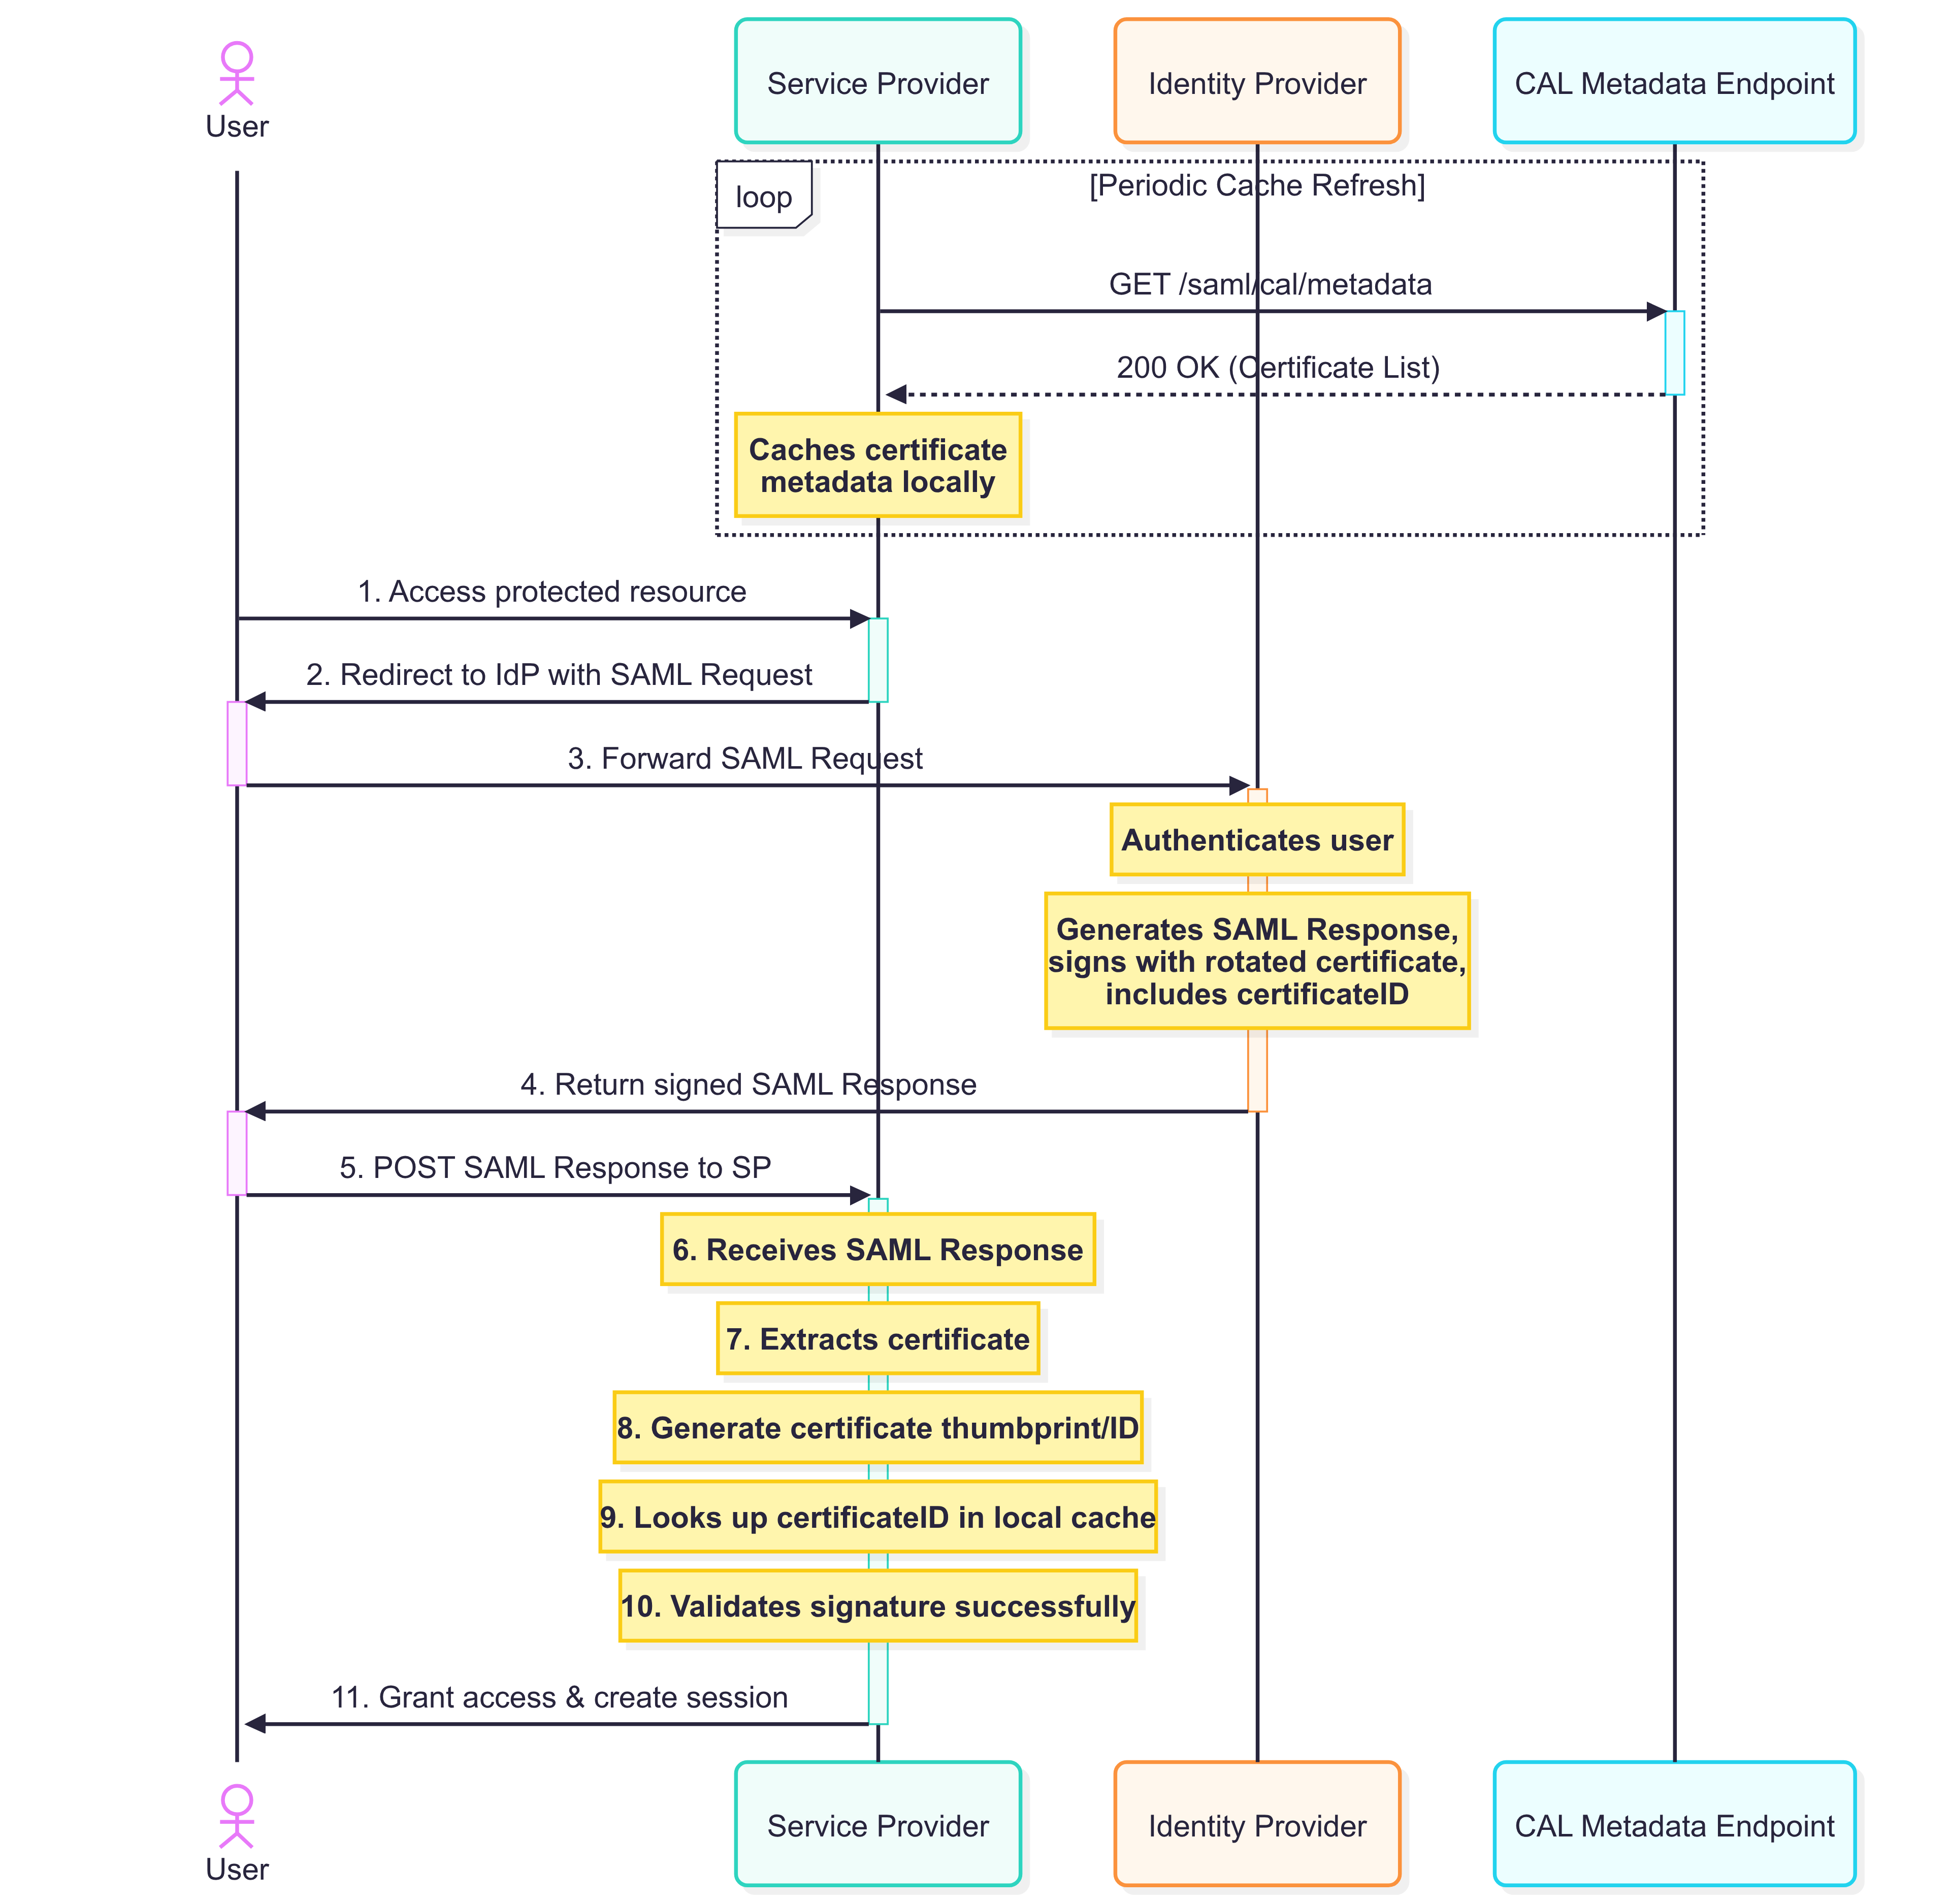
\includegraphics[width=0.9\textwidth]{cal-flow.png}
    \caption{The Certificate Abstraction Layer (CAL) Authentication Flow, showing both background caching and the SSO process.}
    \label{fig:cal-flow}
\end{figure}

\textbf{SP Validation:}  
SP generates a certificate thumbprint using the embedded certificate in the SAML Response, encodes it to base64 (uppercase), and matches it against locally stored \texttt{certificateID}. If validation succeeds, the SP uses the certificate for assertion verification; otherwise, an error is raised.

\textbf{Caching on SPs:}  
SPs periodically sync certificate metadata from IdPs and cache it locally. This reduces the need for frequent endpoint lookups, improving latency and performance in high-throughput federation setups.

\textbf{Federation Metadata Extensions:}  
Extend \texttt{KeyDescriptor} entries to include CAL-specific properties directly in metadata, enabling federations to declare support for dynamic certificate management seamlessly.

\subsection*{Example Metadata Schema Snippet:}
\begin{verbatim}
<Certificates>
    <Certificate>
        <Alias>DefaultCert</Alias>
        <Thumbprint>AB34CD56...</Thumbprint>
        <Base64Thumbprint>QUIzNENENTY...</Base64Thumbprint>
        <Version>1.2</Version>
        <Expires>2025-12-31</Expires>
    </Certificate>
    ...
</Certificates>
<KeyDescriptor>
    <SupportedFeatures>
        <Feature>CAL</Feature>
    </SupportedFeatures>
</KeyDescriptor>
\end{verbatim}

\section*{Benefits}
\begin{itemize}
    \item \textbf{Effortless Key Rotation:} Certificate references (\texttt{certificateID}) decouple SP configurations from certificates, making rotation transparent and automated.
    \item \textbf{Improved Reliability:} Centralized metadata and caching mechanisms reduce misconfiguration risk and downtime during rotations.
    \item \textbf{Futureproof Federation:} Federation metadata extensibility aligns with evolving enterprise requirements.
    \item \textbf{Onboarding Agility:} Automation reduces onboarding times for new applications by eliminating static configurations.
    \item \textbf{Enhanced Compliance:} Frequent cryptographic updates become feasible without risking service disruptions.
\end{itemize}

\section*{Backward Compatibility and Migration Strategy}
\begin{itemize}
    \item \textbf{Dual-Mode Support:} SPs continue to operate with legacy configurations while being enhanced incrementally to support CAL features.
    \item \textbf{Graceful Fallback:} SPs default to the mapped certificate when the \texttt{certificateID} field is absent or unsupported.
    \item \textbf{Extensible Metadata:} Federations optionally declare CAL support in metadata while maintaining backward compatibility for older systems.
\end{itemize}

\section*{Path Forward to SAML 3.0}
The proposed enhancements to SAML 2.0, particularly the Certificate Abstraction Layer (CAL), represent substantial improvements in certificate agility, federation scalability, and automation capabilities. While the enhancements function well as optional extensions to SAML 2.0 metadata, they also highlight the need for evolving SAML to address modern challenges such as dynamic federation workflows, multi-cloud deployments, and frequent cryptographic updates.

To encourage adoption and collaboration:
\begin{itemize}
    \item \textbf{Engage with Industry Leaders:} Collaborate with major Identity Providers (IdPs) such as Okta, PingFederate, and ADFS, along with key open-source initiatives like Shibboleth and SimpleSAMLphp, to pilot and refine these enhancements.
    \item \textbf{Consultation with Standards Committees:} Explore opportunities for dialogue with the OASIS technical committee overseeing SAML standards to position CAL as a potential candidate for future inclusion, either as optional metadata extensions or as part of broader protocol evolution.
    \item \textbf{Community Education:} Advocate CAL through detailed whitepapers, presentations, implementation guides, and pilot use cases to demonstrate its feasibility and value in real-world enterprise environments.
\end{itemize}

Through collaboration and practical adoption, CAL could evolve into a cornerstone of agile, scalable, and automation-friendly federations across the identity ecosystem.\\

\section*{Conclusion}
The Certificate Abstraction Layer (CAL) simplifies certificate management, reduces administrative effort, and fosters agility in enterprise federations. By introducing dynamic certificate resolution, caching, and federation metadata extensibility, CAL enhances reliability and scalability while maintaining backward compatibility with existing SAML 2.0 implementations.

\textbf{Call to Action:} Stakeholders and industry experts should collaborate to pilot these enhancements, refine their implementations, and advocate for standardization to push SAML toward its next evolution, ensuring it remains a robust identity federation protocol for modern enterprises. \\ \\ \\ \\ \\ \\ \\ \\ \\ \\ \\ \\


\appendix
\section*{Appendix: License}

\noindent
© 2025 Pushkar Raj \textless\href{mailto:pushkarraj9099@gmail.com}{pushkarraj9099@gmail.com}\textgreater. \\
ORCID: \href{https://orcid.org/0009-0002-8444-0136}{0009-0002-8444-0136}\\
This white paper is licensed under a 
\href{https://creativecommons.org/licenses/by/4.0/}{Creative Commons Attribution 4.0 International License (CC BY 4.0)}.

\medskip

\noindent
You are free to:
\begin{itemize}
  \item \textbf{Share} — copy and redistribute the material in any medium or format
  \item \textbf{Adapt} — remix, transform, and build upon the material for any purpose, even commercially
\end{itemize}

\noindent
Under the following terms:
\begin{itemize}
  \item \textbf{Attribution} — You must give appropriate credit, provide a link to the license, and indicate if changes were made. You may do so in any reasonable manner, but not in any way that suggests the licensor endorses you or your use.
\end{itemize}

\end{document}
